% ============================================================
% HPTU Nueva Sede — Presentación para Tomadores de Decisión
% 30 minutos · Narrativa ejecutiva · Datos contundentes
% Compilar con: lualatex hptu-junta-directiva.tex
% ============================================================
\documentclass[aspectratio=169, 11pt]{beamer}

% ── Tema ────────────────────────────────────────────────────
\usetheme{default}
\usecolortheme{default}
\setbeamertemplate{navigation symbols}{}
\setbeamertemplate{footline}{%
  \hfill\insertframenumber\,/\,\inserttotalframenumber\hspace{6pt}\vspace{4pt}%
}

% Paleta HPTU
\definecolor{hptu}{HTML}{00549F}
\definecolor{hptudark}{HTML}{003D75}
\definecolor{teal}{HTML}{0D9488}
\definecolor{coral}{HTML}{EF4444}
\definecolor{amber}{HTML}{F59E0B}
\definecolor{slate}{HTML}{64748B}
\definecolor{bglight}{HTML}{F8FAFC}
\definecolor{green}{HTML}{22C55E}
\definecolor{violet}{HTML}{8B5CF6}

\setbeamercolor{frametitle}{fg=hptu}
\setbeamercolor{title}{fg=white}
\setbeamercolor{subtitle}{fg=white!85}
\setbeamercolor{author}{fg=white!80}
\setbeamercolor{date}{fg=white!70}
\setbeamercolor{normal text}{fg=black!85}
\setbeamercolor{structure}{fg=hptu}
\setbeamercolor{itemize item}{fg=teal}
\setbeamercolor{itemize subitem}{fg=hptu}
\setbeamercolor{block title}{fg=white, bg=hptu}
\setbeamercolor{block body}{bg=bglight}
\setbeamercolor{block title alerted}{fg=white, bg=coral}
\setbeamercolor{block body alerted}{bg=coral!5}
\setbeamercolor{block title example}{fg=white, bg=teal}
\setbeamercolor{block body example}{bg=teal!5}

\setbeamerfont{frametitle}{size=\Large, series=\bfseries}
\setbeamerfont{title}{size=\Huge, series=\bfseries}
\setbeamerfont{subtitle}{size=\large}
\setbeamertemplate{itemize items}[circle]

% ── Paquetes ────────────────────────────────────────────────
\usepackage{fontspec}
\usepackage{booktabs}
\usepackage{tabularx}
\usepackage{colortbl}
\usepackage{graphicx}
\usepackage{tikz}
\usetikzlibrary{calc, positioning, shapes.geometric, arrows.meta, backgrounds}
\usepackage{pgfplots}
\pgfplotsset{compat=1.18}
\usepackage{multicol}
\usepackage{hyperref}

% Fuentes
\setsansfont{Helvetica Neue}[
  BoldFont={Helvetica Neue Bold},
  ItalicFont={Helvetica Neue Italic},
]

\newcommand{\highlight}[1]{\textcolor{teal}{\textbf{#1}}}
\newcommand{\danger}[1]{\textcolor{coral}{\textbf{#1}}}
\newcommand{\src}[1]{\par\vspace{2pt}{\tiny\textcolor{slate}{Fuente: #1}}}

% ── Metadata ────────────────────────────────────────────────
\title{Nueva Sede HPTU}
\subtitle{Estudio de Localización Estratégica}
\author{Equipo de Análisis Estratégico}
\date{7 de marzo, 2026}

\begin{document}

% ============================================================
% 1. PORTADA
% ============================================================
{
\setbeamercolor{background canvas}{bg=hptu}
\begin{frame}[plain]
\vfill
\begin{center}
{\usebeamerfont{title}\usebeamercolor[fg]{title}\inserttitle}

\vspace{10pt}
{\usebeamerfont{subtitle}\usebeamercolor[fg]{subtitle}\insertsubtitle}

\vspace{20pt}
\begin{tikzpicture}
  \draw[white, line width=0.5pt] (0,0) -- (8,0);
\end{tikzpicture}

\vspace{14pt}
{\small\textcolor{white!80}{
3.8 millones de registros $\cdot$ 15 fuentes oficiales $\cdot$ Cero estimaciones}}

\vspace{6pt}
{\small\textcolor{white!60}{
5 zonas evaluadas $\cdot$ Modelo financiero preliminar $\cdot$ 12 capas interactivas}}

\vspace{20pt}
{\footnotesize\usebeamercolor[fg]{author}\insertdate}
\end{center}
\vfill
\end{frame}
}

% ============================================================
% 2. EL PROBLEMA — 2 min
% ============================================================
{
\setbeamercolor{background canvas}{bg=coral!3}
\begin{frame}{El problema: un hospital saturado, lejos de su mercado}

\begin{columns}[T]
\column{0.52\textwidth}
\vspace{6pt}
\begin{center}
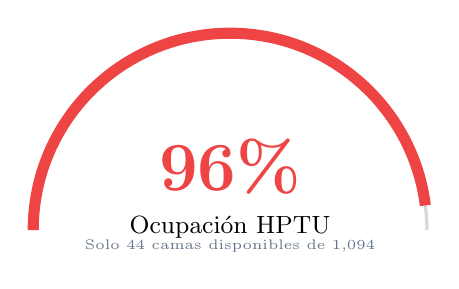
\begin{tikzpicture}
  % Occupancy gauge
  \draw[gray!30, very thick] (0,0) arc (180:0:2.5);
  \draw[coral, line width=4pt] (0,0) arc (180:7.2:2.5);
  \node[font=\Huge\bfseries, coral] at (2.5, 0.8) {96\%};
  \node[font=\small, below] at (2.5, 0.3) {Ocupación HPTU};
  \node[font=\tiny\color{slate}] at (2.5, -0.2) {Solo 44 camas disponibles de 1,094};
\end{tikzpicture}
\end{center}

\vspace{8pt}
El HPTU opera en \textbf{Robledo} con 1,094 camas. Mientras tanto:

\vspace{4pt}
\begin{itemize}\small
  \item \highlight{174,543 predios} de estratos 5 y 6 se concentran en \textbf{El Poblado y Las Palmas}
  \item Están a \danger{más de 20 minutos} del hospital
  \item El corredor Las Palmas tiene \danger{exactamente 0 camas} de alta complejidad
  \item \highlight{103,913 habitantes} sin cobertura hospitalaria a 2037
\end{itemize}

\column{0.45\textwidth}
\begin{alertblock}{\small El déficit es real}
\footnotesize
La OMS recomienda \textbf{3--5 camas} por cada 1,000 habitantes.

\vspace{4pt}
\begin{tabular}{@{}lc@{}}
\toprule
\textbf{Municipio} & \textbf{Camas/1000} \\
\midrule
\rowcolor{coral!10}
Medellín & \danger{1.0} \\
\rowcolor{coral!8}
Envigado & \danger{0.6} \\
Itagüí & \danger{0.6} \\
Sabaneta & \danger{0.5} \\
\midrule
\textbf{OMS mínimo} & \highlight{3.0} \\
\bottomrule
\end{tabular}
\end{alertblock}

\vspace{6pt}
\begin{exampleblock}{\small La pregunta}
\centering\normalsize
\textbf{¿Dónde debe estar\\la nueva sede?}
\end{exampleblock}
\end{columns}
\end{frame}
}

% ============================================================
% 3. METODOLOGÍA — 1 min
% ============================================================
\begin{frame}{Cómo respondemos: datos, no opiniones}

\begin{columns}[T]
\column{0.58\textwidth}
\vspace{4pt}
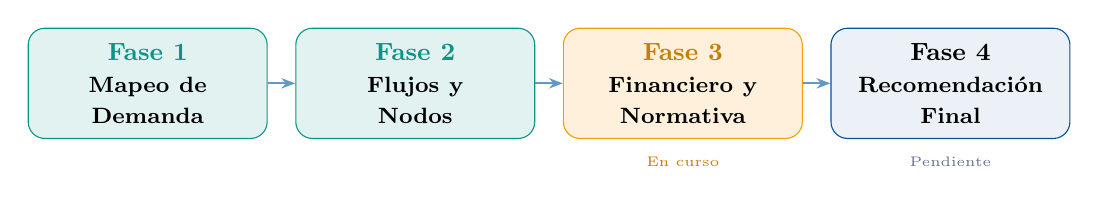
\begin{tikzpicture}[
  node distance=0.35cm,
  phase/.style={draw=hptu, fill=hptu!8, rounded corners=6pt,
                text width=2.8cm, minimum height=1.4cm, align=center,
                font=\small\bfseries},
  done/.style={phase, fill=teal!12, draw=teal},
  active/.style={phase, fill=amber!15, draw=amber},
  arrow/.style={-{Stealth[length=5pt]}, thick, hptu!60}
]
\node[done] (p1) {\textcolor{teal}{Fase 1}\\[2pt]\footnotesize Mapeo de\\Demanda};
\node[done, right=of p1] (p2) {\textcolor{teal}{Fase 2}\\[2pt]\footnotesize Flujos y\\Nodos};
\node[active, right=of p2] (p3) {\textcolor{amber!80!black}{Fase 3}\\[2pt]\footnotesize Financiero y\\Normativa};
\node[phase, right=of p3] (p4) {Fase 4\\[2pt]\footnotesize Recomendación\\Final};

\draw[arrow] (p1) -- (p2);
\draw[arrow] (p2) -- (p3);
\draw[arrow] (p3) -- (p4);

\node[below=3pt of p1, font=\tiny\color{teal}] {\checkmark};
\node[below=3pt of p2, font=\tiny\color{teal}] {\checkmark};
\node[below=3pt of p3, font=\tiny\color{amber!80!black}] {En curso};
\node[below=3pt of p4, font=\tiny\color{slate}] {Pendiente};
\end{tikzpicture}

\vspace{12pt}
Cada zona se evalúa con un \textbf{score de 0 a 100}:

\vspace{6pt}
{\small
$\text{Score} = \underbrace{A \times 35\%}_{\text{Accesibilidad}} + \underbrace{D \times 30\%}_{\text{Demanda}} + \underbrace{C \times 20\%}_{\text{Competencia}} + \underbrace{V \times 15\%}_{\text{Valor Inmob.}}$
}

\column{0.39\textwidth}
\begin{block}{\small Escala del análisis}
\footnotesize
\begin{tabular}{@{}lr@{}}
\toprule
Fuentes primarias & \textbf{15} \\
Registros procesados & \textbf{3.8M+} \\
Zonas evaluadas & \textbf{5} \\
Variables DENSURBAM & \textbf{59} \\
Capas mapa interactivo & \textbf{12} \\
IPS georreferenciadas & \textbf{145} \\
Barrios analizados & \textbf{22} \\
Periodo de datos & 2017--2037 \\
\bottomrule
\end{tabular}
\end{block}

\vspace{4pt}
{\footnotesize Todas las fuentes son datasets oficiales (Catastro, REPS, MEData, DANE, POT) con trazabilidad completa.}
\end{columns}
\end{frame}

% ============================================================
% 4. EL MERCADO OBJETIVO — 2 min
% ============================================================
\begin{frame}{El mercado: 174,543 predios E5/E6 en 22 barrios}

\begin{columns}[T]
\column{0.50\textwidth}
{\scriptsize
\begin{tabular}{@{}lrrl@{}}
\toprule
\textbf{Barrio} & \textbf{Predios E5/E6} & \textbf{\% E5/E6} & \textbf{Avalúo prom.} \\
\midrule
\rowcolor{teal!8}
\textbf{El Poblado core} & \textbf{38,415} & \textbf{98\%} & \$371M \\
Castropol & 6,228 & 97\% & \$327M \\
Manila & 2,144 & 96\% & \$305M \\
Los Balsos No.\ 1 & 4,019 & 95\% & \$401M \\
San Lucas & 3,671 & 93\% & \$512M \\
\rowcolor{teal!6}
Altos del Poblado & 1,867 & 91\% & \$245M \\
El Tesoro & 1,856 & 89\% & \$258M \\
Los Balsos No.\ 2 & 2,143 & 88\% & \$347M \\
{\tiny + 14 barrios más} & & & \\
\midrule
\textbf{Total 22 barrios} & \textbf{174,543} & & \\
\bottomrule
\end{tabular}
}

\vspace{4pt}
\src{Catastro Municipal Medellín (bp59-rj8r), 1,041,413 predios}

\vspace{6pt}
{\footnotesize El corredor Las Palmas concentra \textbf{barrios con 88--98\%} de predios E5/E6 y avalúos promedio de \highlight{\$245M--\$512M COP}. Alta capacidad de pago.}

\column{0.47\textwidth}
\begin{exampleblock}{\small Perfil del mercado}
\footnotesize
\begin{itemize}
  \item \textbf{Prepagada/póliza}: SURA Salud El Poblado tiene \highlight{320,000 afiliados}
  \item \textbf{Colegios premium}: Colombo Británico, Montessori, Marymount, Columbus --- 30 instituciones generan tráfico cautivo de familias E5/E6
  \item \textbf{Clubes}: El Rodeo, Campestre Medellín --- red social de referidos
  \item \textbf{Corporativo}: Milla de Oro, Bancolombia HQ (4,000 empleados con prepagada)
\end{itemize}
\end{exampleblock}

\vspace{4pt}
\begin{alertblock}{\small 0 camas para este mercado}
\footnotesize Ningún hospital en el corredor ofrece \textbf{trasplantes, hematología avanzada ni oncología compleja}. El HPTU sería el \textbf{único referente} de alta complejidad.
\end{alertblock}
\end{columns}
\end{frame}

% ============================================================
% 5. LA BRECHA — 3 min
% ============================================================
{
\setbeamercolor{background canvas}{bg=coral!3}
\begin{frame}{La brecha: un corredor sin hospital de alta complejidad}

\begin{columns}[T]
\column{0.48\textwidth}
\textbf{Red hospitalaria actual}:

\vspace{4pt}
{\scriptsize
\begin{tabular}{@{}lrcl@{}}
\toprule
\textbf{Hospital} & \textbf{Camas} & \textbf{Ocup.} & \textbf{Dist.} \\
\midrule
\rowcolor{coral!10}
HPTU Robledo & 1,094 & \danger{96\%} & 8.5 km \\
Cl.\ Medellín & 624 & 88\% & 3.2 km \\
\rowcolor{coral!6}
HGM ESE & 384 & \danger{92\%} & 7+ km \\
Cl.\ del Prado & 304 & 85\% & 5+ km \\
Cl.\ CES & 213 & 82\% & \danger{7.16 km} \\
H.\ Uribe Ángel & 120 & 78\% & 4+ km \\
\midrule
\textbf{Total sistema} & \textbf{2,739} & \textbf{91\%} & \\
\bottomrule
\end{tabular}
}

\vspace{4pt}
{\scriptsize\textcolor{coral}{$\blacktriangledown$} Cl.\ CES verificada: está en \textbf{Prado Centro}, NO en Las Palmas (Google Geocoding API).}

\vspace{4pt}
\begin{block}{\small En el corredor Las Palmas}
\footnotesize
\begin{tabular}{@{}lcc@{}}
Cl.\ Rosario Tesoro & 158 camas & \footnotesize sin trasplantes \\
Cl.\ Las Vegas & 171 camas & \footnotesize sin oncología \\
\end{tabular}

\vspace{3pt}
\danger{0 camas} de alta complejidad.
\end{block}

\column{0.49\textwidth}
\textbf{DENSURBAM confirma} (Variable 49 --- IRS Salud):

\vspace{4pt}
\begin{center}
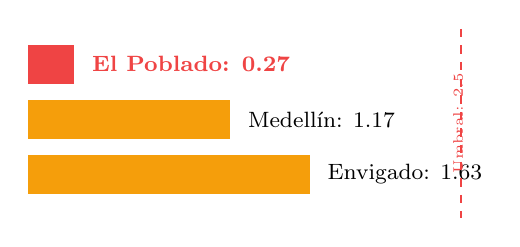
\begin{tikzpicture}
  \fill[coral] (0,0) rectangle (0.27/2.5*5.5, 0.5);
  \node[right, font=\footnotesize\bfseries] at (0.27/2.5*5.5+0.1, 0.25) {\danger{El Poblado: 0.27}};

  \fill[amber] (0,-0.7) rectangle (1.17/2.5*5.5, -0.2);
  \node[right, font=\footnotesize] at (1.17/2.5*5.5+0.1, -0.45) {Medellín: 1.17};

  \fill[amber] (0,-1.4) rectangle (1.63/2.5*5.5, -0.9);
  \node[right, font=\footnotesize] at (1.63/2.5*5.5+0.1, -1.15) {Envigado: 1.63};

  \draw[coral, thick, dashed] (2.5/2.5*5.5, 0.7) -- (2.5/2.5*5.5, -1.7);
  \node[font=\tiny, coral, rotate=90, anchor=south] at (2.5/2.5*5.5+0.15, -0.5) {Umbral: 2.5};
\end{tikzpicture}
\end{center}

\vspace{2pt}
{\scriptsize\textcolor{slate}{DENSURBAM (URBAM-EAFIT/AMVA), 59 variables, proy.\ 2037}}

\vspace{4pt}
\textbf{10 barrios} del corredor tienen \danger{0.0 m²} de oferta de salud.

\vspace{3pt}
{\footnotesize
\begin{tabular}{@{}lr@{}}
Población sin cobertura 2037 & \danger{103,913 hab} \\
Infraestructura requerida & \danger{363,696 m²} \\
\end{tabular}
}

\vspace{4pt}
{\footnotesize Serán \highlight{+152,000 personas más} en el área focal para 2037. El sistema \textbf{no tiene capacidad} para absorber ese crecimiento.}
\end{columns}
\end{frame}
}

% ============================================================
% 6. EL TRÁFICO — 2 min
% ============================================================
\begin{frame}{El tráfico: Las Palmas fluye, El Poblado colapsa}

\begin{columns}[T]
\column{0.50\textwidth}
Con \highlight{682,502 observaciones} de MEData (2017--2020):

\vspace{4pt}
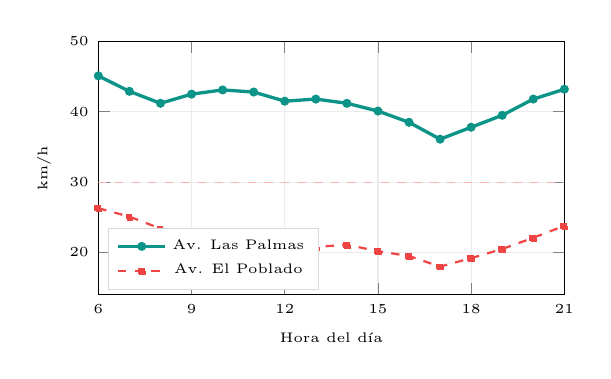
\begin{tikzpicture}
\begin{axis}[
  width=7.5cm, height=4.8cm,
  xlabel={\tiny Hora del día},
  ylabel={\tiny km/h},
  xmin=6, xmax=21, ymin=14, ymax=50,
  xtick={6,9,12,15,18,21},
  xticklabel style={font=\tiny},
  yticklabel style={font=\tiny},
  grid=major, grid style={gray!15},
  legend style={at={(0.02,0.02)}, anchor=south west, font=\tiny,
               fill=white, draw=gray!30},
]
\addplot[teal, very thick, mark=*, mark size=1pt] coordinates {
  (6,45.1)(7,42.9)(8,41.2)(9,42.5)(10,43.1)(11,42.8)
  (12,41.5)(13,41.8)(14,41.2)(15,40.1)(16,38.5)(17,36.1)
  (18,37.8)(19,39.5)(20,41.8)(21,43.2)
};
\addlegendentry{Av. Las Palmas}
\addplot[coral, thick, dashed, mark=square*, mark size=1pt] coordinates {
  (6,26.3)(7,25.1)(8,23.4)(9,22.8)(10,21.9)(11,21.2)
  (12,20.5)(13,20.8)(14,21.1)(15,20.2)(16,19.5)(17,18.0)
  (18,19.2)(19,20.5)(20,22.1)(21,23.8)
};
\addlegendentry{Av. El Poblado}
\addplot[coral!40, thin, dashed] coordinates {(6,30)(21,30)};
\end{axis}
\end{tikzpicture}

\src{MEData Velocidad Tiempo Viaje GT (7t5n-3b3w)}

\column{0.47\textwidth}
\vspace{8pt}
A las \textbf{5:00 PM} (hora pico):

\vspace{4pt}
\begin{alertblock}{}
\centering
{\Large \danger{18.0 km/h}}\\
\footnotesize Av.\ El Poblado --- congestión severa
\end{alertblock}

\vspace{2pt}
\begin{exampleblock}{}
\centering
{\Large \highlight{36.1 km/h}}\\
\footnotesize Av.\ Las Palmas --- \textbf{100\% más rápido}
\end{exampleblock}

\vspace{6pt}
{\footnotesize\textbf{Desde 6 orígenes} a Las Palmas Bajo:}

\vspace{3pt}
{\scriptsize
\begin{tabular}{@{}lrl@{}}
Milla de Oro & \highlight{15.4 min} & Google \\
El Poblado & \highlight{17.7 min} & Google \\
Envigado & 24.8 min & Google \\
Laureles & 32.3 min & Mapbox \\
Itagüí & 33.4 min & Mapbox \\
\midrule
\textbf{Promedio} & \textbf{26.6 min} & \\
\end{tabular}
}

\vspace{4pt}
{\scriptsize El \textbf{80\% del mercado E5/E6} llega en menos de 25 min.}
\end{columns}
\end{frame}

% ============================================================
% 7. LAS 5 ZONAS — 2 min
% ============================================================
\begin{frame}{Cinco zonas evaluadas: el ranking}

\begin{center}
{\small Modelo MCDA: Accesibilidad (35\%) + Demanda (30\%) + Competencia (20\%) + Valor Inmobiliario (15\%)}
\end{center}

\vspace{6pt}
\begin{center}
{\small
\begin{tabular}{@{}lccccccc@{}}
\toprule
\textbf{Zona candidata} & \textbf{Acc.} & \textbf{Dem.} & \textbf{Comp.} & \textbf{Valor} & \textbf{SCORE} & \textbf{min HPTU} & \textbf{POT} \\
 & {\tiny 35\%} & {\tiny 30\%} & {\tiny 20\%} & {\tiny 15\%} & & & \\
\midrule
\rowcolor{teal!12}
\textbf{Las Palmas Bajo} & \textbf{92} & \textbf{93} & \textbf{78} & \textbf{80} & \highlight{88} & 23.8 & 9/9 \\
Las Palmas Medio & 72 & 84 & 82 & 70 & 77 & 31.8 & 6/9 \\
Envigado--Zúñiga & 75 & 80 & 62 & 74 & 74 & 22.4 & --- \\
N.\ Poblado--Itagüí & 82 & 68 & 52 & 58 & 67 & 19.0 & --- \\
\rowcolor{coral!6}
Las Palmas Alto & 42 & 52 & 90 & 62 & 58 & \danger{57.1} & N/A \\
\bottomrule
\end{tabular}
}
\end{center}

\vspace{8pt}
\begin{columns}[T]
\column{0.32\textwidth}
\begin{exampleblock}{\small \#1 Las Palmas Bajo}
\footnotesize \textbf{Única zona} con score $>$80 en las \textbf{4 dimensiones}. Equilibrio perfecto entre demanda, accesibilidad y viabilidad POT.
\end{exampleblock}

\column{0.32\textwidth}
\begin{block}{\small \#2 Las Palmas Medio}
\footnotesize Pierde \textbf{11 puntos} por accesibilidad (+8 min a HPTU). Más suelo disponible (132K m²) pero menor demanda cercana.
\end{block}

\column{0.32\textwidth}
\begin{alertblock}{\small \#5 Las Palmas Alto}
\footnotesize \danger{Descartado}: 57 min a HPTU, aislamiento geográfico, suelo rural. Inviable operativa y financieramente.
\end{alertblock}
\end{columns}
\end{frame}

% ============================================================
% 8. RECOMENDACIÓN — 3 min
% ============================================================
{
\setbeamercolor{background canvas}{bg=teal!3}
\begin{frame}{Recomendación: Las Palmas Bajo — Score 88/100}

\begin{columns}[T]
\column{0.42\textwidth}
\textbf{Ubicación}: Altos del Poblado / El Tesoro\\
{\footnotesize Entre Indiana y la EIA, después del cuello de botella de tráfico}

\vspace{8pt}
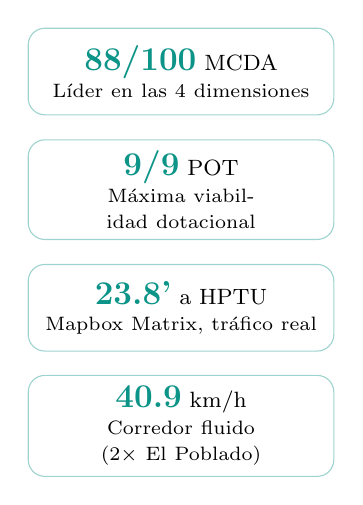
\begin{tikzpicture}[
  pillar/.style={draw=teal!40, fill=white, rounded corners=6pt,
                 text width=3.6cm, minimum height=1.1cm, align=center,
                 font=\footnotesize, inner sep=4pt},
]
\node[pillar] (p1) at (0,0) {
  {\large\textcolor{teal}{\textbf{88/100}}} MCDA\\{\scriptsize Líder en las 4 dimensiones}
};
\node[pillar] (p2) at (0,-1.5) {
  {\large\textcolor{teal}{\textbf{9/9}}} POT\\{\scriptsize Máxima viabilidad dotacional}
};
\node[pillar] (p3) at (0,-3.0) {
  {\large\textcolor{teal}{\textbf{23.8'}}} a HPTU\\{\scriptsize Mapbox Matrix, tráfico real}
};
\node[pillar] (p4) at (0,-4.5) {
  {\large\textcolor{teal}{\textbf{40.9}}} km/h\\{\scriptsize Corredor fluido (2$\times$ El Poblado)}
};
\end{tikzpicture}

\column{0.55\textwidth}
{\footnotesize
\begin{tabular}{@{}p{3.8cm}l@{}}
\toprule
\textbf{Parámetro} & \textbf{Valor} \\
\midrule
Elevación & $\sim$1,700 msnm \\
Predios E5/E6 en Comuna 14 & \highlight{38,415} \\
Avalúo promedio zona & \$245M COP \\
POT CL\_D (carga dotacional) & 2.38 \\
Suelo potencial disponible & 68,020 m² \\
Altura máxima POT & 11.7 pisos \\
Cl.\ más cercana (Rosario) & 0.93 km / 158 camas \\
A Cl.\ Las Vegas & 10.5 min \\
A Milla de Oro & 10.7 min \\
A CC El Tesoro & 10.4 min \\
Competidores alta complej. & \danger{0 en el corredor} \\
\bottomrule
\end{tabular}
}

\vspace{6pt}
\begin{exampleblock}{\small ¿Por qué esta zona y no otra?}
\footnotesize Es la \textbf{única} que combina: (1) demanda masiva a menos de 15 min, (2) corredor de tráfico fluido, (3) viabilidad POT máxima, (4) cero competencia de alta complejidad, y (5) VPN positivo.
\end{exampleblock}
\end{columns}
\end{frame}
}

% ============================================================
% 9. MODELO FINANCIERO — 3 min
% ============================================================
\begin{frame}{Modelo financiero: factibilidad por zona}

\begin{columns}[T]
\column{0.52\textwidth}
{\footnotesize
\begin{tabular}{@{}l r r r r@{}}
\toprule
\textbf{Zona} & \textbf{Camas} & \textbf{Inversión} & \textbf{Payback} & \textbf{VPN 10y} \\
\midrule
\rowcolor{teal!10}
\textbf{LP Bajo} & \textbf{250} & \textbf{\$90MM} & \textbf{11.3y} & \highlight{+\$4.8MM} \\
LP Medio & 300 & \$108MM & 9.4y & +\$15.3MM \\
Envigado & 220 & \$82MM & 11.3y & +\$4.0MM \\
N.\ Poblado & 260 & \$98MM & 9.6y & +\$14.7MM \\
\rowcolor{coral!8}
LP Alto & 150 & \$55MM & \danger{22.9y} & \danger{--\$31MM} \\
\bottomrule
\end{tabular}
}
{\tiny Cifras en miles de millones COP. WACC 12\%, ramp-up 60\%/80\%/100\% años 1/2/3+.}

\vspace{6pt}
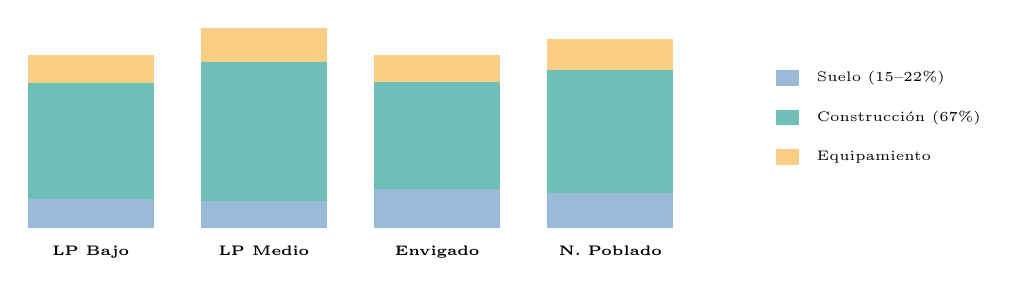
\begin{tikzpicture}
  \foreach \x/\label/\land/\const/\equip in {
    0/LP Bajo/15/60/15,
    2.2/LP Medio/14/72/18,
    4.4/Envigado/20/56/14,
    6.6/N. Poblado/18/64/16} {
    \pgfmathsetmacro{\landh}{\land/90*2.2}
    \pgfmathsetmacro{\consth}{\const/90*2.2}
    \pgfmathsetmacro{\equiph}{\equip/90*2.2}
    \fill[hptu!40] (\x,0) rectangle (\x+1.6, \landh);
    \fill[teal!60] (\x,\landh) rectangle (\x+1.6, \landh+\consth);
    \fill[amber!50] (\x,\landh+\consth) rectangle (\x+1.6, \landh+\consth+\equiph);
    \node[font=\tiny\bfseries, below] at (\x+0.8, -0.1) {\label};
  }
  \fill[hptu!40] (9.5,1.8) rectangle (9.8,2.0); \node[font=\tiny, right] at (9.9,1.9) {Suelo (15--22\%)};
  \fill[teal!60] (9.5,1.3) rectangle (9.8,1.5); \node[font=\tiny, right] at (9.9,1.4) {Construcción (67\%)};
  \fill[amber!50] (9.5,0.8) rectangle (9.8,1.0); \node[font=\tiny, right] at (9.9,0.9) {Equipamiento};
\end{tikzpicture}

\column{0.45\textwidth}
\begin{block}{\small Parámetros base}
\scriptsize
\begin{tabular}{@{}ll@{}}
Construcción/m² & \$4.0M {\tiny(Scielo/U.\ Militar)} \\
Dotación & 25\% {\tiny(DNP)} \\
Ocupación & 80\% {\tiny(estándar)} \\
Ingreso/cama/año & \$1,600M {\tiny(HUSI)} {\color{coral}$\blacktriangledown$} \\
EBITDA & 8\% {\color{coral}$\blacktriangledown$} \\
WACC & 12\% {\color{coral}$\blacktriangledown$} \\
Timeline total & 54 meses (4.5 años) \\
\end{tabular}
\end{block}

\vspace{4pt}
\begin{exampleblock}{\small Hallazgo clave}
\footnotesize El suelo = solo \textbf{15--22\%} del total. La diferencia de precio entre zonas importa \textbf{menos} que el tamaño del lote y la altura POT.
\end{exampleblock}

\vspace{3pt}
\begin{alertblock}{\small Sensibilidad}
\footnotesize Si ingreso/cama = \$2,000M (privado premium, +25\%), VPN de LP Bajo sube a \highlight{+\$25MM}. Este es el parámetro \textbf{más sensible}.
\end{alertblock}
\end{columns}
\end{frame}

% ============================================================
% 10. VIABILIDAD POT — 2 min
% ============================================================
\begin{frame}{Viabilidad normativa: el POT respalda la ubicación}

\begin{columns}[T]
\column{0.50\textwidth}
Análisis POT de \textbf{22 barrios} del corredor:

\vspace{6pt}
{\scriptsize
\begin{tabular}{@{}lcccr@{}}
\toprule
\textbf{Barrio} & \textbf{Score} & \textbf{CL\_D} & \textbf{Pisos} & \textbf{Suelo (m²)} \\
\midrule
\rowcolor{teal!10}
\textbf{Altos del Poblado} & \highlight{9/9} & 2.38 & 11.7 & 68,020 \\
\rowcolor{teal!6}
El Tesoro & 9/9 & 2.52 & 7.2 & 119,482 \\
Castropol & 8/9 & 1.89 & 7.1 & 65,591 \\
Los Balsos No.\ 1 & 8/9 & 2.15 & 11.5 & 97,440 \\
\midrule
Los Balsos No.\ 2 & 6/9 & & 16.7 & 132,161 \\
Las Lomas No.\ 1 & 5/9 & & 15.4 & 30,281 \\
Las Lomas No.\ 2 & 5/9 & & 20.0 & --- \\
\midrule
{\tiny + 15 barrios más} & 1--7 & & & \\
\bottomrule
\end{tabular}
}

\vspace{3pt}
\src{POT Batería Indicadores (3ciz-tpgr), Acuerdo 48 de 2014}

\vspace{4pt}
{\footnotesize CL\_D = Carga Localizada Dotacional. Valores $>$2.0 = \textbf{aptos para uso dotacional} (hospitales, equipamientos de salud).}

\column{0.47\textwidth}
\begin{exampleblock}{\small Altos del Poblado: máxima viabilidad}
\footnotesize
\begin{itemize}
  \item CL\_D = \highlight{2.38} (muy por encima del umbral)
  \item ICS = 57.4 (capacidad de soporte)
  \item ICF = 2.78 (carga de flujos favorable)
  \item Suelo potencial: \highlight{68,020 m²}
  \item Altura máxima: 11.7 pisos (suficiente para 250 camas)
\end{itemize}
\end{exampleblock}

\vspace{4pt}
\begin{block}{\small Viabilidad por categoría}
\footnotesize
\begin{tabular}{@{}lcl@{}}
\textcolor{green}{$\bullet$} & ALTA (8--9) & 4 barrios \\
\textcolor{teal}{$\bullet$} & MEDIA-ALTA (6--7) & 6 barrios \\
\textcolor{amber}{$\bullet$} & MEDIA (4--5) & 7 barrios \\
\textcolor{coral}{$\bullet$} & BAJA (1--3) & 5 barrios \\
\end{tabular}
\end{block}

\vspace{4pt}
{\footnotesize\textcolor{coral}{$\blacktriangledown$} Pendiente: fichas normativas \textbf{específicas por polígono} (DAP Medellín) para confirmar IO/IC del lote.}
\end{columns}
\end{frame}

% ============================================================
% 11. CRECIMIENTO POBLACIONAL — 2 min
% ============================================================
\begin{frame}{La demanda crecerá: +152,000 personas al 2037}

\begin{columns}[T]
\column{0.50\textwidth}
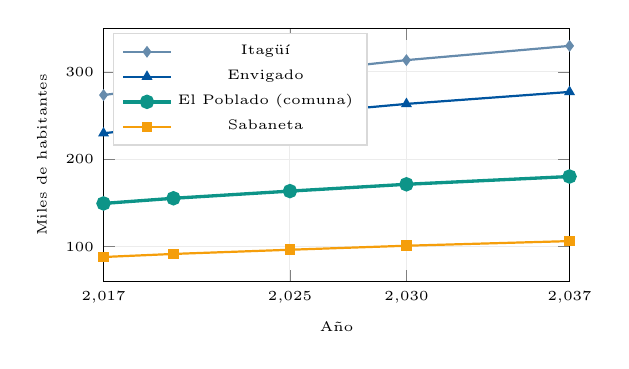
\begin{tikzpicture}
\begin{axis}[
  width=7.5cm, height=4.8cm,
  xlabel={\tiny Año},
  ylabel={\tiny Miles de habitantes},
  xmin=2017, xmax=2037, ymin=60, ymax=350,
  xtick={2017,2025,2030,2037},
  xticklabel style={font=\tiny},
  yticklabel style={font=\tiny},
  grid=major, grid style={gray!15},
  legend style={at={(0.02,0.98)}, anchor=north west, font=\tiny,
               fill=white, draw=gray!30},
]
\addplot[hptudark!60, thick, mark=diamond*, mark size=1.5pt] coordinates {
  (2017,273.5)(2020,284.1)(2025,299.2)(2030,313.5)(2037,329.8)
};
\addlegendentry{Itagüí}
\addplot[hptu, thick, mark=triangle*, mark size=1.5pt] coordinates {
  (2017,229.8)(2020,238.7)(2025,251.4)(2030,263.4)(2037,277.1)
};
\addlegendentry{Envigado}
\addplot[teal, very thick, mark=*, mark size=2pt] coordinates {
  (2017,149.5)(2020,155.4)(2025,163.6)(2030,171.4)(2037,180.3)
};
\addlegendentry{El Poblado (comuna)}
\addplot[amber, thick, mark=square*, mark size=1.5pt] coordinates {
  (2017,88.2)(2020,91.7)(2025,96.5)(2030,101.1)(2037,106.4)
};
\addlegendentry{Sabaneta}
\end{axis}
\end{tikzpicture}

\src{DENSURBAM (DANE + AMVA), modelo tendencial 2017--2037}

\column{0.47\textwidth}
\vspace{6pt}
{\footnotesize
\begin{tabular}{@{}lrrl@{}}
\toprule
\textbf{Área} & \textbf{2017} & \textbf{2037} & \textbf{Crecim.} \\
\midrule
El Poblado & 149K & 180K & +20.6\% \\
Envigado & 230K & 277K & +20.6\% \\
Itagüí & 274K & 330K & +20.6\% \\
Sabaneta & 88K & 106K & +20.6\% \\
\midrule
\textbf{Área focal} & \textbf{741K} & \textbf{893K} & \\
\bottomrule
\end{tabular}
}

\vspace{6pt}
\begin{alertblock}{\small La ecuación}
\footnotesize
\begin{tabular}{@{}l@{}}
Red hospitalaria al \danger{91\% de ocupación} \\
\textbf{+ 152,000 personas más} \\
\textbf{+ 0 camas nuevas en el corredor} \\
\midrule
= \danger{Colapso del sistema} \\
\end{tabular}

\vspace{4pt}
La nueva sede no es una oportunidad de mercado. Es una \textbf{necesidad de infraestructura}.
\end{alertblock}
\end{columns}
\end{frame}

% ============================================================
% 12. PLATAFORMA INTERACTIVA — 1 min
% ============================================================
\begin{frame}{Plataforma interactiva: toda la evidencia en un mapa}

\begin{columns}[T]
\column{0.50\textwidth}
\textbf{12 capas de datos} en un tablero interactivo:

\vspace{6pt}
{\footnotesize
\begin{tabular}{@{}lrl@{}}
\toprule
\textbf{Capa} & \textbf{Datos} & \textbf{Fuente} \\
\midrule
Red de salud & 145 IPS & REPS \\
Catastro E5/E6 & 22 barrios & Catastro \\
Viabilidad POT & 22 barrios & POT \\
Tráfico por tramo & 8 segmentos & MEData \\
Colegios corredor & 30 POIs & OSM \\
Comercio corredor & 28 POIs & OSM \\
Isocronas & 10/20/30 min & Mapbox \\
Rutas alternas & 6 rutas & Mapbox \\
Zonas candidatas & 5 zonas & MCDA \\
Corredor Las Palmas & geometría & Mapbox \\
Estratos 5/6 & polígonos & ArcGIS \\
POIs clave & 27 puntos & Verificados \\
\bottomrule
\end{tabular}
}

\column{0.47\textwidth}
\vspace{6pt}
\begin{block}{\small Funcionalidades}
\footnotesize
\begin{itemize}
  \item Toggle on/off por capa individual
  \item Click en cualquier punto = popup con datos
  \item Clustering dinámico (IPS)
  \item Estilos de mapa: claro, oscuro, satélite
  \item Panel detallado por zona candidata
  \item Leyenda colapsible
\end{itemize}
\end{block}

\vspace{4pt}
\begin{exampleblock}{\small Acceso}
\centering
\small \url{https://hptu-localizacion.vercel.app}

\vspace{4pt}
\footnotesize Disponible en cualquier navegador.\\
Todos los datos son interactivos.
\end{exampleblock}

\vspace{4pt}
{\scriptsize\textcolor{slate}{Incluye también: dashboard financiero, análisis de brecha, gráficas de tráfico, sección DENSURBAM y fuentes con trazabilidad.}}
\end{columns}
\end{frame}

% ============================================================
% 13. SUPUESTOS POR VALIDAR — 2 min
% ============================================================
{
\setbeamercolor{background canvas}{bg=coral!3}
\begin{frame}{Lo que falta: 8 parámetros por validar}

{\footnotesize
\begin{tabular}{@{}p{4.0cm}ccl@{}}
\toprule
\textbf{Parámetro} & \textbf{Prior.} & \textbf{Valor actual} & \textbf{Fuente de validación} \\
\midrule
\rowcolor{coral!8}
Precio suelo/m² por zona & \danger{ALTA} & \$0.5--2.5M/m² & Lonja de Propiedad Raíz Medellín \\
\rowcolor{coral!8}
Ingreso/cama/año & \danger{ALTA} & \$1,600M COP & Cl.\ Pablo Tobón, Las Américas \\
\rowcolor{coral!6}
Margen EBITDA operativo & \danger{ALTA} & 8\% & Supersalud (estados financieros) \\
Fichas normativas POT & \danger{ALTA} & Estimadas & DAP Medellín / GeoMedellín \\
Lotes disponibles por zona & \danger{ALTA} & 8--15K m² & Inmobiliarias del corredor \\
\rowcolor{amber!10}
WACC del proyecto & MEDIA & 12\% & Análisis banca de inversión \\
\rowcolor{amber!10}
Costos diseño + licencias & MEDIA & 18 meses est. & Firmas de arquitectura hospitalaria \\
IO/IC específico por lote & MEDIA & Estimados & Fichas normativas POT \\
\bottomrule
\end{tabular}
}

\vspace{8pt}
\begin{columns}[T]
\column{0.48\textwidth}
\begin{alertblock}{\small Sensibilidad del modelo}
\footnotesize El ingreso por cama/año es el parámetro \textbf{más sensible}:

\vspace{3pt}
{\scriptsize
\begin{tabular}{@{}lcc@{}}
\toprule
\textbf{Escenario} & \textbf{Ingreso/cama} & \textbf{VPN LP Bajo} \\
\midrule
\rowcolor{coral!6}
Conservador (HUSI) & \$1,600M & +\$4.8MM \\
\rowcolor{teal!6}
Privado premium & \$2,000M & \highlight{+\$25MM} \\
Privado alto & \$2,200M & +\$38MM \\
\bottomrule
\end{tabular}
}
\end{alertblock}

\column{0.48\textwidth}
\begin{block}{\small Riesgos identificados}
\footnotesize
\begin{enumerate}\scriptsize
  \item Demoras en licenciamiento POT
  \item Volatilidad costos de construcción
  \item Cartera EPS ($\sim$\$14B COP sector)
  \item Nuevos competidores en el corredor
  \item Cambios regulatorios (POT/salud)
\end{enumerate}
\end{block}
\end{columns}
\end{frame}
}

% ============================================================
% 14. PRÓXIMOS PASOS — 2 min
% ============================================================
\begin{frame}{Ruta a la decisión: Fases 3 y 4}

\begin{columns}[T]
\column{0.50\textwidth}
\textbf{Fase 3 --- Profundización} {\small(en curso)}

\vspace{4pt}
\begin{enumerate}\footnotesize
  \item[\textcolor{teal}{1.}] \textbf{Validar modelo financiero}\\
    {\scriptsize Lonja de Propiedad Raíz, Supersalud, benchmark hospitales privados}
  \item[\textcolor{teal}{2.}] \textbf{Due diligence POT}\\
    {\scriptsize Fichas normativas específicas por polígono (DAP Medellín)}
  \item[\textcolor{teal}{3.}] \textbf{Identificar lotes}\\
    {\scriptsize Búsqueda activa con inmobiliarias, contacto propietarios}
  \item[\textcolor{teal}{4.}] \textbf{Competencia detallada}\\
    {\scriptsize Servicios premium, especialidades, tarifas por zona}
  \item[\textcolor{teal}{5.}] \textbf{Análisis de sensibilidad}\\
    {\scriptsize Monte Carlo o escenarios sobre parámetros críticos}
\end{enumerate}

\vspace{6pt}
\textbf{Fase 4 --- Recomendación Final}

\vspace{4pt}
\begin{enumerate}\footnotesize
  \item[\textcolor{hptu}{1.}] Informe ejecutivo final (PDF/web)
  \item[\textcolor{hptu}{2.}] Shortlist de 2--3 lotes específicos
  \item[\textcolor{hptu}{3.}] Presentación a Junta Directiva
  \item[\textcolor{hptu}{4.}] Análisis de escenarios para decisión
\end{enumerate}

\column{0.47\textwidth}
\begin{block}{\small Entregables del estudio}
\footnotesize
\begin{enumerate}
  \item \textbf{Plataforma web} interactiva con 12 capas\\
    {\scriptsize hptu-localizacion.vercel.app}
  \item \textbf{Informe técnico} PDF con metodología completa
  \item \textbf{Base georreferenciada} (15 GeoJSON + datos)
  \item \textbf{Dashboard MCDA} con scoring por zona
  \item \textbf{Modelo financiero} con análisis de sensibilidad
\end{enumerate}
\end{block}

\vspace{4pt}
\begin{exampleblock}{\small Referencia sectorial}
\footnotesize El modelo de \textbf{San Vicente Rionegro} validó que una expansión estratégica hacia la población objetivo funciona. Las Palmas Bajo sigue esa misma lógica: acercar la alta complejidad al mercado E5/E6.
\end{exampleblock}
\end{columns}
\end{frame}

% ============================================================
% 15. FUENTES — 1 min (referencia)
% ============================================================
\begin{frame}{Fuentes primarias: 15 datasets, 3.8M+ registros}

\vspace{2pt}
{\scriptsize
\begin{tabular}{@{}p{4.0cm}lrp{5.5cm}@{}}
\toprule
\textbf{Fuente} & \textbf{Dataset} & \textbf{Registros} & \textbf{Uso} \\
\midrule
Catastro Municipal Medellín & bp59-rj8r & 1,041,413 & Predios E5/E6, avalúos, barrio \\
DENSURBAM (URBAM/EAFIT) & densurbam.com.co & 1,220,415 & IRS salud, sostenibilidad, proy.\ 2037 \\
MEData Velocidades & 7t5n-3b3w & 682,502 & Velocidades por corredor 2017--2020 \\
POT Bat.\ Indicadores & 3ciz-tpgr & 331,741 & CL\_D, ICS, alturas, suelo potencial \\
Lotes Potenciales & m4wi-nn8x & 441,966 & 592 lotes en corredor Las Palmas \\
MEData Aforos & b9s9-jw7c & 74,900 & Volúmenes vehiculares por hora \\
Licencias Urbanísticas & pxmc-bbtu & 32,266 & 27 licencias dotacional/salud \\
REPS Prestadores & b4dp-ximh & 1,536 & IPS habilitadas, camas, complejidad \\
REPS Capacidad Inst.\ & s2ru-bqt6 & 1,711 & Camas por tipo, nov.\ 2022 \\
DANE CNPV 2018 & evm3-92yw & 465 & Población por municipio \\
OSM Overpass API & Overpass QL & 1,323 & 178 salud, 750 educación, 330 comercio \\
Mapbox Matrix/Directions & API v1 & 40 & Tiempos reales, isocronas, rutas \\
Google Routes API & Routes v2 & 12 & Validación cruzada tiempos \\
ArcGIS Estratos & FeatureServer & 5,142 & Manzanas censales por estrato \\
EPM Cobertura & datos.gov.co & 951 & Suscriptores E6 por comuna \\
\bottomrule
\end{tabular}
}

\vspace{6pt}
\begin{center}
{\small\textbf{Total: 3,836,371+ registros} de fuentes oficiales. Cero estimaciones. Todo trazable.}
\end{center}
\end{frame}

% ============================================================
% 16. SÍNTESIS EJECUTIVA
% ============================================================
{
\setbeamercolor{background canvas}{bg=hptu!3}
\begin{frame}{Síntesis ejecutiva}

\begin{center}
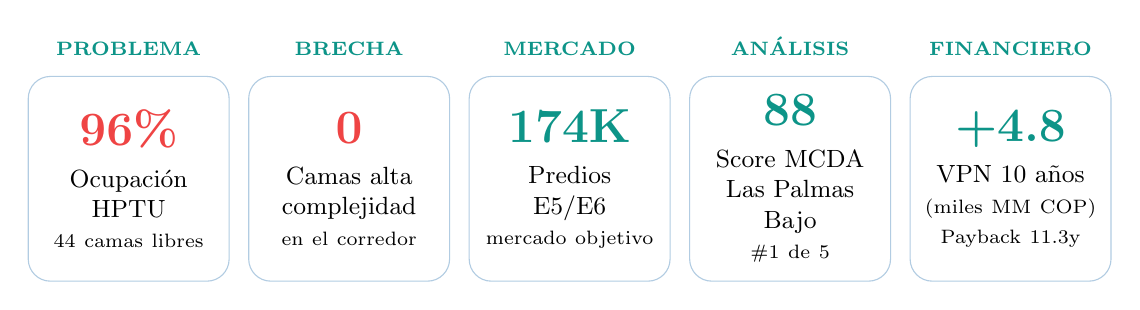
\begin{tikzpicture}[
  pillar/.style={draw=hptu!30, fill=white, rounded corners=8pt,
                 text width=2.2cm, minimum height=2.6cm, align=center,
                 font=\small, inner sep=5pt},
  plabel/.style={font=\scriptsize\bfseries, teal},
]
\node[pillar] (p1) at (0,0) {
  {\LARGE\textcolor{coral}{\textbf{96\%}}}\\[4pt]
  Ocupación\\HPTU\\{\scriptsize 44 camas libres}
};
\node[pillar] (p2) at (2.8,0) {
  {\LARGE\textcolor{coral}{\textbf{0}}}\\[4pt]
  Camas alta\\complejidad\\{\scriptsize en el corredor}
};
\node[pillar] (p3) at (5.6,0) {
  {\LARGE\textcolor{teal}{\textbf{174K}}}\\[4pt]
  Predios\\E5/E6\\{\scriptsize mercado objetivo}
};
\node[pillar] (p4) at (8.4,0) {
  {\LARGE\textcolor{teal}{\textbf{88}}}\\[4pt]
  Score MCDA\\Las Palmas\\Bajo\\{\scriptsize \#1 de 5}
};
\node[pillar] (p5) at (11.2,0) {
  {\LARGE\textcolor{teal}{\textbf{+4.8}}}\\[4pt]
  VPN 10 años\\{\scriptsize (miles MM COP)}\\{\scriptsize Payback 11.3y}
};

\node[plabel, above=4pt of p1] {PROBLEMA};
\node[plabel, above=4pt of p2] {BRECHA};
\node[plabel, above=4pt of p3] {MERCADO};
\node[plabel, above=4pt of p4] {ANÁLISIS};
\node[plabel, above=4pt of p5] {FINANCIERO};
\end{tikzpicture}
\end{center}

\vspace{8pt}
\begin{columns}[T]
\column{0.48\textwidth}
\begin{exampleblock}{\small Lo que los datos dicen}
\footnotesize
\begin{enumerate}
  \item El sistema está \textbf{saturado} y crecerá +152K personas
  \item El corredor tiene \textbf{0 camas} de alta complejidad
  \item Las Palmas Bajo es la \textbf{única zona} con score $>$80 en las 4 dimensiones
  \item El proyecto es \textbf{financieramente viable} (VPN positivo en 4 de 5 zonas)
\end{enumerate}
\end{exampleblock}

\column{0.48\textwidth}
\begin{alertblock}{\small La decisión pendiente}
\footnotesize Para pasar de \textbf{recomendación} a \textbf{decisión de inversión}:

\vspace{3pt}
\begin{enumerate}
  \item Validar 5 supuestos financieros de alta prioridad
  \item Confirmar fichas normativas POT específicas
  \item Identificar 2--3 lotes concretos
  \item Completar análisis de sensibilidad
\end{enumerate}

\vspace{3pt}
{\scriptsize Esto es la Fase 3. Estamos en ella.}
\end{alertblock}
\end{columns}
\end{frame}
}

% ============================================================
% 17. CIERRE
% ============================================================
{
\setbeamercolor{background canvas}{bg=hptu}
\begin{frame}[plain]
\vfill
\begin{center}
{\Huge\bfseries\textcolor{white}{¿Preguntas?}}

\vspace{20pt}
\begin{tikzpicture}
  \draw[white, line width=0.5pt] (0,0) -- (8,0);
\end{tikzpicture}

\vspace{16pt}
{\large\textcolor{white!90}{HPTU — Nueva Sede}}

\vspace{6pt}
{\normalsize\textcolor{white!80}{Estudio de Localización Estratégica}}

\vspace{14pt}
{\small\textcolor{white!70}{Plataforma interactiva:}}\\
{\small\textcolor{white!90}{\url{https://hptu-localizacion.vercel.app}}}

\vspace{10pt}
{\small\textcolor{white!60}{15 fuentes oficiales $\cdot$ 3.8M+ registros $\cdot$ 12 capas interactivas}}

\vspace{6pt}
{\small\textcolor{white!60}{5 zonas evaluadas $\cdot$ Modelo financiero preliminar}}

\vspace{20pt}
{\footnotesize\textcolor{white!40}{Todo es datos. Nada es opinión.}}
\end{center}
\vfill
\end{frame}
}

\end{document}
